\section{Literature Review}
\label{sec:lit}

% ---- Talking points written up as prose (your version: 04_literature_review_draft.tex).

This review seeks to articulate the gap in the literature for partial shading that the aims and objectives of the project seek to fill. Analysing how it defeats a conventional maximum power point tracker (\cref{sec:lit_shading}). Exploring the differential power processing converters that are proposed to recover the lost energy (\cref{sec:lit_dpp}). Discovers how converters of this kind have been controlled (\cref{sec:lit_control}). the modelling, simulation and test methods used to develop them (\cref{sec:lit_methods}). Finally, identifying the gap this project fills (\cref{sec:gap}).

\subsection{Partial shading and MPPT}
\label{sec:lit_shading}
At its core a solar controller is a maximum power point tracker (MPPT): a buck or boost stage whose duty is adjusted so that the array operates at its point of highest power. The MPPT literature is mature. Esram and Chapman catalogue 19 tracking methods \cite{esram_comparison_2007}, and Sarvi and Azadian update the field into classical, bio-inspired and machine-learning classes \cite{sarvi_comprehensive_2022}. Most of these methods assume that the power--voltage (P--V) curve of the array has a single peak.

Partial shading breaks that assumption \cite{belhaouas_pv_2017,bingol_analysis_2018,mehedi_critical_2021}. Every module in a series string carries the same current, so a shaded module either limits the string current to what it can produce or, once its bypass diode conducts, drops out of the string altogether. Each combination of conducting and bypassed modules gives the P--V curve its own peak. \Cref{fig:pvmismatch} shows this for the four-module string model built in Semester 1. For a scenario of three modules at 1000\,W/m$^2$ and one module at 500\,W/m$^2$ the string offers 1656\,W with that module bypassed or about 1240\,W with all four conducting. For a graduated shading scenario four separate peaks appear, with the global maximum of 914\,W at only 78\,V. A conventional perturb-and-observe (P\&O) tracker climbs whichever peak it starts nearest and is trapped there \cite{riquelme-dominguez_systematic_2022}. Even a tracker that finds the global maximum leaves energy behind: \cref{tab:pvshading} compares each string's global maximum with the sum of its modules' individual maximum power points, and the mismatch loss reaches 34\,\% under graduated shading.

\begin{figure}[htbp]
  \centering
  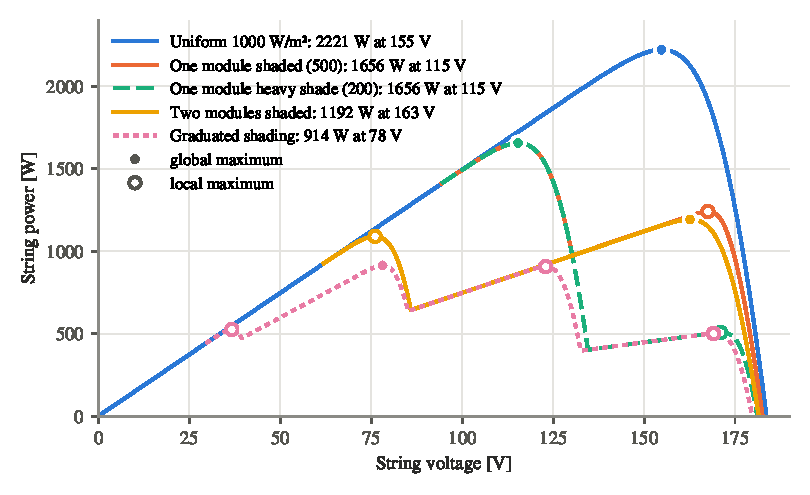
\includegraphics[width=0.85\linewidth]{misc/pv_shading}
  \caption{P--V curves of a four-module string (AIKO Neostar A555, single-diode model with bypass diodes) under five irradiance patterns.}
  \label{fig:pvmismatch}
\end{figure}

\begin{table}[htbp]
  \centering
  \small
  \caption[{Mismatch loss of the shaded strings}]{Mismatch loss of the shaded strings in \cref{fig:pvmismatch}: string global maximum against the sum of the modules' individual maxima (the power a lossless per-module tracker could extract).}
  \label{tab:pvshading}
  \begin{tabular}{l c r r r}
    \toprule
    Scenario & Irradiance [W/m$^2$] & Module MPPs [W] & String MPP [W] & Loss \\
    \midrule
    Uniform                 & 1000, 1000, 1000, 1000 & 2221 & 2221 & 0.0\,\% \\
    One module shaded       & 1000, 1000, 1000, 500  & 1944 & 1656 & 14.8\,\% \\
    One module heavy shade  & 1000, 1000, 1000, 200  & 1775 & 1656 & 6.7\,\% \\
    Two modules shaded      & 1000, 1000, 500, 500   & 1667 & 1193 & 28.5\,\% \\
    Graduated shading       & 1000, 800, 500, 200    & 1388 & 914  & 34.1\,\% \\
    \bottomrule
  \end{tabular}
\end{table}

Array reconfiguration (series-parallel, bridge-linked and total-cross-tied) reduces this mismatch loss but cannot remove it \cite{rao_maximum_2014}. Bypass diodes protect the shaded cells, but at the cost of a multi-peaked P--V curve and the energy of every bypassed module. Recovering that energy requires moving power between the modules themselves.

\subsection{Existing shuffler concepts: DPP and S-PPC}
\label{sec:lit_dpp}
The power shuffler is part of the family of differential power processors (DPP) \cite{kasper_classification_2014}, whose reason for being is to move differences in power around a system, effectively balancing out either voltage or current. The serial partial power converter (S-PPC) specialises in moving the power differentials of modules that are connected in series \cite{jeong_segmented_2020}.

The idea has a long history at QUT: Walker, Xue and Sernia first proposed per-module ``shuffling'' converters that let each module in a string operate at its own maximum power point \cite{walker_pv_2003}. Hui's later QUT work documents why this matters outside the lab \cite{hui_development_2020}. Shufflers of a very different design were fitted to ATN's solar car \emph{Priscilla} for the 2019 Bridgestone World Solar Challenge. IN a prestigious challenge such as this every watt matters. The curvature of the 1.25\,kW array and obstacles passing overhead shade it unevenly while driving. Drops in performance of these solar panels translate to reduced speed and cruise time in this endurance race. The design was rushed into the car under tight timelines with limited testing, the devices did not perform reliably and ultimately failed during the challenge, and the follow-on work was redirected to making them operate safely and reliably. It is a clear reminder that protection and safety features have to be designed into a shuffler from the start (\cref{sec:risks}). Kasper et al.\ classify panel-integrated DC--DC concepts and identify the buck-boost as the most promising \cite{kasper_classification_2014,kasper_impact_2014}. Olalla et al.\ formalise the modelling of DPP architectures and show near-ideal energy extraction with converter ratings that scale with the mismatch rather than the string power \cite{olalla_modeling_2014,olalla_performance_2014}. Jeong et al.\ review DPP architectures \cite{jeong_review_2018} and demonstrate a four-unit segmented DPP experimentally \cite{jeong_segmented_2020}; Li and Cobos give a framework for comparing the VA ratings of partial power converters \cite{li_classification_2021}; and dos Santos et al.\ present a practical two-switch S-PPC \cite{dos_santos_two-switch_2021}. A common thread runs through these works: their focus is the power stage and the architecture, and the control is either not discussed or kept simple and classical, with a PI loop on a single unit.

The S-PPC used in this project is the interleaved buck-boost converter: two half-bridge legs joined through a coupled inductor to the midpoint between two series modules (\cref{fig:shuffler}). At a duty of $D=0.5$ the midpoint sits at half the pair voltage; moving $D$ away from 0.5 moves current from one module to the other, and in steady state the current circulating between the two phases should be zero.

\subsection{Controlling the interleaved buck-boost}
\label{sec:lit_control}
A single buck-boost converter is described by one second-order ordinary differential equation (ODE), and classical frequency-domain design works well for it. Interleaving changes this the presence of a second phase and the coupled inductance couple the states (ie. PV module voltages and the currents through each inductor winding), so they cannot be controlled independently \cite{milasi_robust_2024}. Kabalci and Boyar add an extended Kalman filter to an interleaved boost converter to handle these coupled states \cite{kabalci_highly_2022}, and the behaviour of coupled inductors in interleaved converters is treated in \cite{huang_high-frequency_2015,guacci_experimental_2019}.

State-space methods handle this coupling naturally. Batzelis et al.\ give a six-state representation of irradiance-driven PV dynamics that includes the boost converter, the PI integrator and the MPPT reference \cite{batzelis_state-space_2018}; this is the modelling style adopted here, extended with the shuffler's winding dynamics. Other state-space MPPT work reports that LQR and LQR-PI controllers outperform P\&O \cite{lin_state-space_2021,khan_state-space_2024,assabaa_enhancing_2025}.

\subsection{Modelling, simulation and test methods}
\label{sec:lit_methods}
Switching converters are normally designed for control with averaged models. State-space averaging replaces the switched circuit with a continuous-time model whose inputs are the duty cycles \cite{middlebrook_general_1976}, and Kassakian et al.\ develop averaged and linearised models of the buck-boost family as the basis for its control design \cite{kassakian_principles_2024}. Averaging discards the switching ripple, so the model is valid only well below the switching frequency, and it says nothing about dead time, sampling delay or sensor noise.

The simulation tools follow from those two limits. Simulink is the standard environment for model-based design: the controller and an averaged plant run together in one model, which makes it the natural tool for model-in-the-loop (MIL) verification on the left of the V-model \cite{mathworks_simulink_2026,seal_system_2018}. QSPICE is a switching-level SPICE simulator with built-in C++ compilation, so compiled C code can run as a block inside the circuit \cite{qorvo_qspice_2023}. That allows the firmware's own control core to be tested against real switches, drivers, dead time and sensing models before it reaches hardware, closing the gap the averaged model leaves.

For experimental testing, MPPT performance is standardised: EN~50530 defines dynamic test sequences of irradiance ramps for measuring tracking efficiency, and Li et al.\ use them to compare MPPT algorithms experimentally \cite{li_comparative_2021}. Riquelme-Dom\'inguez and Mart\'inez evaluate MPPT algorithms on state-space models under several such dynamic test procedures \cite{riquelme-dominguez_systematic_2022}. These procedures need a programmable PV simulator. This project draws on the same approach, repeatable steps on the bench with programmable supplies and an electronic load followed by validation on a real string outdoors, but a full EN~50530 campaign is outside its scope.

\subsection{The gap}
\label{sec:gap}
Past controllers have been able to rely on classical methods such as PI because each controls a single converter. Multiple-input multiple-output (MIMO) control of a string of coupled shufflers has had very limited exploration, and control of the interleaved buck-boost converter is itself a niche topic. To the author's knowledge, no published work models an $N$-module string of interleaved buck-boost DPP converters as one MIMO plant, identifies its DC gain matrix and closes a decoupling integral controller on real hardware, with the module-voltage differences and circulating currents as outputs. This project does that, carrying the design through analytical, Simulink, QSPICE, firmware, bench and solar phases, and reports the same metrics for every phase on one set of test cases.
